\subsection{Wire-Fitted Q-Learning}

The $Q$-Learning algorithm had to be immediately modified to be able to work in continuous state-action spaces for it to be suitable for Fido.
Conventional $Q$-Learning is discrete.
No relation is made between states or actions, and every action for each state must be performed individually in a noisy feedback system to determine its $Q$-value.
However, Fido will work in a large, continuous state-action spaces where relations made between (state-action, $Q$-value) pairs can drastically reduce the number of reward iterations needed for convergence.
An example of a task that would benefit from continuity is teaching Fido to adjust the speed of its motors based on the intensity of light that the robot detects.
There is an obvious gradient relation between the (state-action, $Q$-value) pairs in this task and with a limited number of $Q$-values known, it is possible to correctly model $Q$.

To accommodate continuous action-spaces, we coupled a wire-fitted moving least squares interpolator with our feed-forward neural network as described in \cite{gaskett}.

Feed-forward neural networks can generalize between states in $Q$-Learning problems with discrete actions as described in \cite{rummery}.
To extend this implementation to a continuous action space, our feed-forward neural network outputs discrete ``wires'' when given a state.
Each wire consists of an action with its respective $Q$-value for the state given to the neural network.
These wires may be interpolated to model $Q$, allowing us to get the $Q$-value of any action performed in a state given as an input to the network.
The interpolator used in Fido is a wire-fitted moving least squares interpolator used in the context of a memory-based learning system \cite{baird}.

The wire-fitting function calculates $Q$-value of an action $\hat{a}$ for a state $s$ given a set of $n$ actions $a$ each with a respective $Q$-value $q$ as such:

\begin{equation}
	Q(a, s) = \cfrac{\sum_{i=0}^{n}\cfrac{q_i}{||\hat{a}-a_i||^2+c(q_{max}-q_i)+k}}{\sum_{i=0}^{n}\cfrac{1}{||\hat{a}-a_i||^2+c(q_{max}-q_i)+k}}
	\,,
\end{equation}

\noindent
where $q_{max}$ is the greatest $Q$-value among the set of $Q$-values $q$, and $k$ is a small value that avoids division by zero.
$c$ is the smoothing factor.
The greater the smoothing factor, the smoother the interpolated function.


Figure \ref{fig::wirefitexample} is an example of interpolation on a set of wires.
The graph shows the value of one-dimensional actions plotted against their respective $Q$-values.
The wire-fitting function has few properties that make it especially suited for Fido.

\begin{figure}[ht]
   \centering
   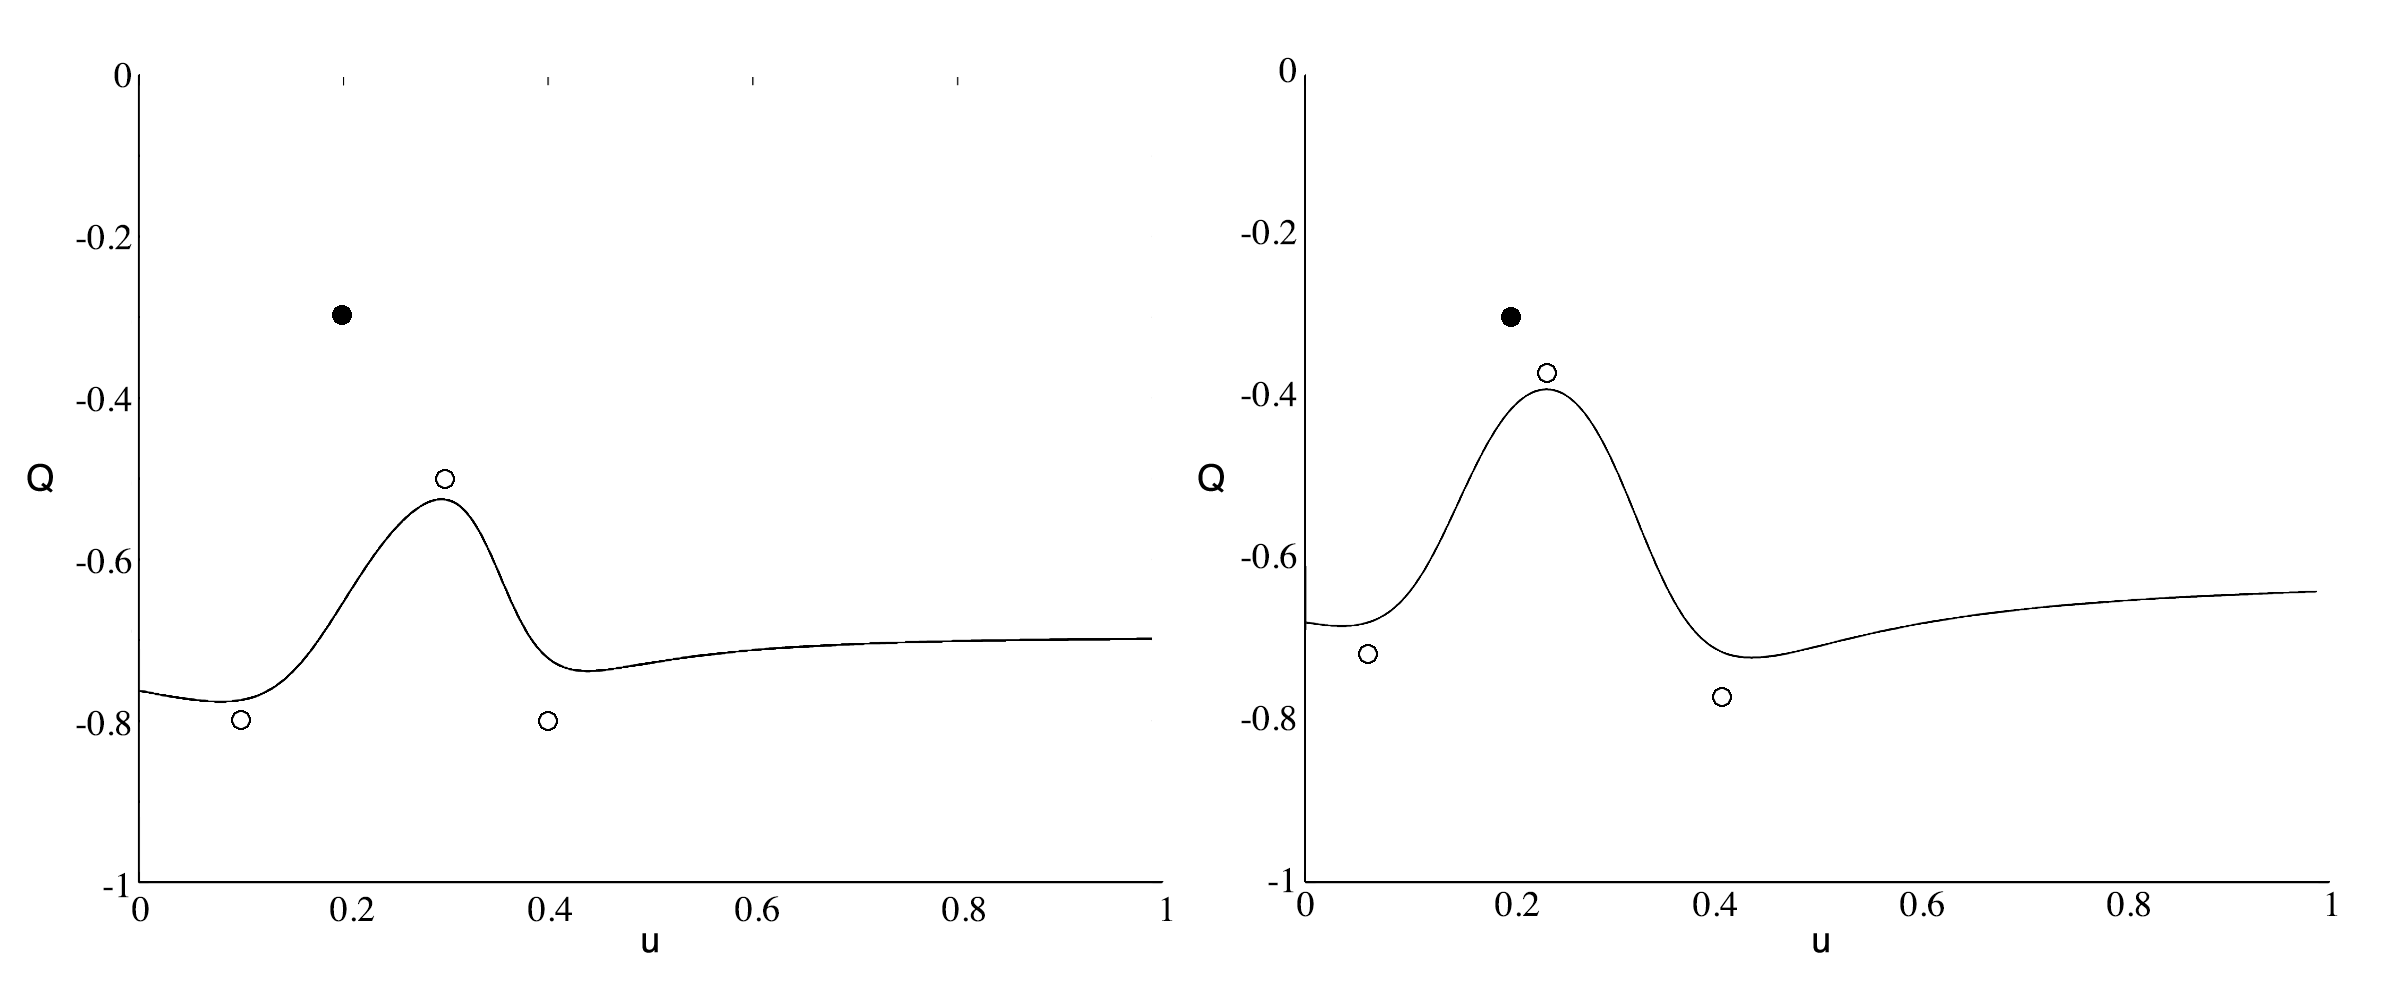
\includegraphics[height=6.5cm]{Figures/WireFit.png}
	\caption{Moving Least Squares Interpolator (adapted from Gaskett, Wettergreen, \& Zelinsky, 1999)}
   \label{fig::wirefitexample}
\end{figure}

Every update to the $Q$-value requires that $q_{max}$ is computed and the action that produces $q_{max}$ is needed for common action selection policies.
As proved in \cite{baird}, the wire with the greatest $Q$-value is the interpolation point with the greatest $Q$-value, therefore $q_{max}$ is the maximum $Q$-value out of the set of wires given to the wire-fitting function.
This makes it extremely computationally cheap to compute $Q$-value, allowing Fido's latency to stay minimal.

The wire-fitting function is derivable.
This allows us to update our wires, and therefore our model of $Q$, using gradient descent.
Gradient descent is an optimization algorithm that looks to find the local minimum of a function by modifying each of its parameters, one by one.
The update function for a parameter is calculated as such:

\begin{equation}
	a = a - \gamma \Delta F(a)
	\,,
	\label{equ::wirefiterrorfunction}
\end{equation}

where $a$ is the parameter to be updated, $\gamma$ is the learning rate, and $\Delta F(a)$ is the partial derivative of the function to be minimized $F$ with respect to $a$.
In the case of Fido, once the reward and new state for an action-state pair is received and an updated $Q$-value $\hat{q}$ is calculated using Equation \ref{equ::updateqlearn}, we are trying to minimize the wire-fitting function's error at predicting $\hat{q}$ when given the wires for Fido's previous state.
This error can be calculated as:

\begin{equation}
	(\hat{q} - q)^2
	\,,
	\label{equ::wirefiterrorfunction}
\end{equation}

\noindent

where $q$ is the old $Q$-value.
Using Equation \ref{equ::wirefiterrorfunction} as our function to be minimized and the partial derivative of the wire-fitting function with respect to each action vector and each q-value, we may compute the partial derivatives of our cost function.
Using these, new wires may be calculated for Fido's previous state using gradient descent.
Fido's neural network may be trained using back propagation to output these new wires when given the previous state.

\subsection{Uncertainty Value}

Fido calculates the "uncertainty" $u$ of its system. Such a value should lower as Fido learns a task and rise if Fido's task changes. This value is useful in adjusting a number hyperparameters that are detailed in the next few sections, such as the exploratory level of the system. Every learning iteration, after updating its wires using stochastic gradient descent, Fido calculates its uncertainty value as the means squared error between its original set of wires and its newly updated set of wires.

\subsection{Action Selection}

$Q$-learn requires that actions are selected to be performed.
There are a number of approaches to choosing this action, and each has a large affect on the behavior of the learning implementation.
The most common approach is to simply pick the action with the best $Q$-value for the current state.
However this strategy stifles exploration of the state-action space, increasing the time of convergence on a task, hurting the retrain-ability of the model, and giving a bias towards an actor's starting policy, which is random.
This problem is compounded in the case of Fido due to the large state and action spaces that Fido must explore.
Another common method of action selection is to choose each action randomly for a set number of reward iterations, and then to switch to choosing the action with the highest $Q$-value.
This plan improves upon the first by allowing for a period of exploration, but is not suited for Fido.
During its lifetime, Fido must have the ability to learn new tasks and be retrained by the operator providing feedback, and so, must continuously explore its state space.

Fido selects actions probabilistically using a Boltzmann or soft-max distribution of probability.
The likelihood that an action $\hat{a}$ will be chosen from a set of $n$ actions $a$ for a state $s$ is given as:

\begin{equation}
	p(\hat{a}) = \cfrac{e^{\frac{Q(s, \hat{a})}{T}}}{\sum_{i=0}^{n}e^{\frac{Q(s, a_i)}{T}}}
	\,.
	\label{equ::boltzmann}
\end{equation}

$T$ is the temperature, or exploration level.
As $T$ approaches infinity, a random action is chosen.
As $T$ tends toward 0, the best action is chosen.
Fido keeps $T$ at a constant value around $T \approx 0.15$ throughout its lifetime to encourage occasional, continued exploration.

$T$ is set proportional to Fido's uncertainty value, so that Fido rapidly explores when it is first initialized or is being retrained. This allows Fido to converge on tasks in fewer reward iterations than if $T$ were set as a constant. As Fido learns a task, $T$ will approach 0. This means that Fido will accurately perform a task when sure of its actions, increasing Fido's average reward over other systems.

\subsection{Experience Replay}

\subsection{Dynamic Neural Network Architecture}
